\section{Authentication \& Authorization}
\label{sec:auth-authz}

In a hospital environment, access control is not only a technical feature. It directly affects patient safety and privacy. Medical data is highly sensitive, but clinicians also need fast access to the right information to make decisions in time. This creates a difficult balance between confidentiality and availability. In practice, a good security design must support both: it must protect the data from unauthorized access, and it must still allow legitimate staff to access information when care requires it \cite{Shin2015, SantosPereira2013}.
\vspace{0.5cm}


This section introduces two core concepts: authentication and authorization. Authentication is needed to establish who is making a request. Authorization then decides what that requester is allowed to do. In this thesis, the main focus is authorization because it is where access control models such as RBAC and ABAC are applied.



\subsection{Authentication}
\label{subsec:authentication}

Authentication answers a simple question: \textit{“Who are you?”} It is the process used by a system to verify the identity of an entity (a user, a service, or an application). The output of authentication is usually an identity claim that the system trusts enough to continue processing the request.
\vspace{0.5cm}


In healthcare systems, authentication is especially important because the same record may be accessed by many different parties (doctors, nurses, lab staff, administrative staff, and sometimes external institutions). If a system cannot reliably authenticate the requester, then any authorization decision becomes meaningless. In an interoperability scenario, authentication also supports secure communication across domains, where systems may belong to different institutions \cite{SantosPereira2013}.
\vspace{0.5cm}


However, authentication alone does not prevent misuse. A user can be correctly authenticated and still request data that is outside their responsibility. This is why authentication must be followed by authorization.

\subsection{Authorization}
\label{subsec:authorization}

Authorization answers the next question: \textit{“What are you allowed to do?”} After authentication establishes an identity, authorization checks whether that identity is permitted to perform a specific action on a specific resource. In practice, authorization is the core of an access control system.

In healthcare, authorization must support normal clinical workflows and also handle special situations. For example, a physician in the patient’s care team may be allowed to read the patient’s clinical notes, while an administrative staff member may be limited to billing-related data. The challenge is that hospital contexts change frequently. Patients move across departments, staff work in shifts, emergencies happen, and access needs can change within minutes. A system that only supports static rules will either block necessary care or become too permissive.
\vspace{0.5cm}


Many healthcare systems therefore discuss the need to balance confidentiality and availability. A well-known example is emergency override (often described as “break-glass” behavior), where access rules can be overridden in a controlled way, with strong auditing and justification requirements \cite{SantosPereira2013}. This shows an important point: in hospitals, authorization is not just about denying access; it is also about enabling safe access in time-critical cases.
\vspace{0.5cm}


Because authorization is where most complexity lives, this thesis focuses on designing and implementing authorization logic using access control models. The next section introduces the most common models used for authorization decisions.

\section{Access Control Models}
\label{sec:ac-models}

An access control model defines how authorization decisions are made. It describes the policy structure (how permissions are expressed) and the evaluation process (how requests are checked). In healthcare, the most widely deployed approach in real systems is Role-Based Access Control (RBAC), because hospital job functions map naturally to roles such as doctor, nurse, pharmacist, and receptionist \cite{SantosPereira2013}.
\vspace{0.5cm}


However, modern hospital systems also face requirements that do not fit cleanly into roles alone. Many decisions depend on context, such as the current department, time, shift, emergency status, or whether the requester is part of a care team. These issues motivate extensions and hybrid approaches, which will be discussed later in this chapter. This subsection first reviews RBAC, because it is the baseline for most hospital authorization systems.

\subsection{Role-Based Access Control (RBAC)}
\label{subsec:rbac}

Role-Based Access Control (RBAC) is one of the most widely adopted authorization approaches in real organizations because it matches how people and responsibilities are organized in practice. Instead of assigning permissions directly to each individual user, RBAC assigns permissions to \textit{roles}. Users then receive permissions through the roles they hold. This simple idea reduces administrative effort and makes it easier to reason about “who can do what” at an organizational level \cite{Sandhu1996, Ferraiolo2007RBAC2E}.

\begin{figure} [H]
    \centering
    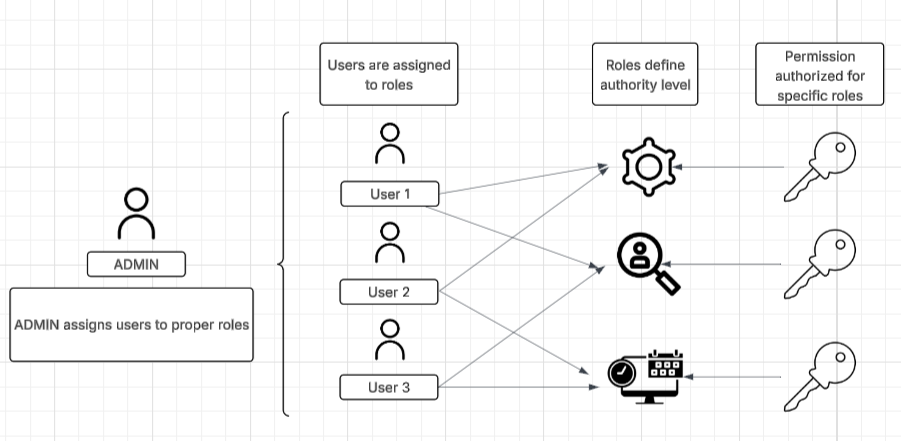
\includegraphics[width=0.75\linewidth]{images/rbac.png}
    \caption{Role-based Access Control}
    \label{fig:rbac}
\end{figure}

This role-driven view fits hospital environments naturally. Hospitals already classify staff by job function and responsibility, such as doctor, nurse, lab technician, or billing staff. When a new staff member joins or changes department, administrators typically think in terms of assigning or removing job functions rather than manually managing hundreds of fine-grained permissions. For this reason, many healthcare systems adopt RBAC as a practical baseline for authorization management \cite{SantosPereira2013, Shin2015}.
\vspace{0.5cm}


To understand RBAC in a concrete way, it helps to follow the typical decision path that a system takes during authorization. After a user is authenticated, the system knows the user identity. RBAC then checks which roles this user has been assigned. Each role represents a set of permissions, where a permission can be understood as an approved operation on a protected resource (for example, \textit{read medical record}, \textit{update lab result}, or \textit{approve discharge}). In daily operation, RBAC often uses the concept of a \textit{session}, where a user activates one or more roles to perform tasks, which supports the principle of least privilege in practice \cite{Sandhu1996, Ferraiolo2007RBAC2E}. In short, RBAC makes authorization decisions by mapping:
\textit{user} $\rightarrow$ \textit{roles} $\rightarrow$ \textit{permissions}.
\vspace{0.5cm}


RBAC also supports more structured control beyond basic role assignment. A common extension is a \textit{role hierarchy}, where senior roles inherit permissions from junior roles. This mirrors real organizational structures (for example, a department head may inherit permissions of a regular physician). RBAC systems can also enforce \textit{constraints}, such as separation of duty, to reduce the risk of misuse and ensure that sensitive workflows cannot be completed by a single user without checks \cite{Sandhu1996, Ferraiolo2007RBAC2E}. These features are particularly relevant in regulated domains like healthcare, where accountability and policy compliance are important \cite{Shin2015}.
\vspace{0.5cm}


However, while RBAC is practical and understandable, hospitals also expose its limitations. Clinical work often depends on \textit{dynamic context}. Access is not decided only by job title. It depends on factors such as whether a doctor is part of the treating team for a particular patient, whether a nurse is on shift and assigned to the same ward, or whether an emergency situation requires controlled override access. A hospital may also classify some records as more sensitive than others, where access rules become stricter \cite{SantosPereira2013}. These conditions change frequently and can be different for the same user across time and location.
\vspace{0.5cm}


When RBAC is used alone, a common response is to create more roles to represent these situations (for example, splitting roles by department, ward, or shift). Over time, this creates an operational burden: the number of roles grows, exceptions accumulate, and policy management becomes harder and more error-prone. In healthcare, this is risky because policy mistakes can either block legitimate care or expose sensitive data \cite{SantosPereira2013, Shin2015}. In addition, emergency access patterns (often described as “break-glass”) show that the system must sometimes allow access outside normal role boundaries while still ensuring strong auditing and justification \cite{SantosPereira2013}. Such requirements are difficult to capture cleanly using roles alone.
\vspace{0.5cm}


For these reasons, RBAC is a strong baseline but not sufficient by itself for fine-grained hospital scenarios. This thesis therefore treats RBAC as the foundation that captures stable organizational responsibilities, and it motivates the need for additional mechanisms that can express context-based conditions in a controlled way. This leads to Attribute-Based Access Control (ABAC) and hybrid RBAC/ABAC approaches, which aim to improve flexibility without losing manageability.


\subsection{Attribute-Based Access Control (ABAC)}
\label{subsec:abac}

RBAC matches the stable structure of a hospital, but many hospital decisions depend on the current situation: which patient is assigned, which ward the staff is working in, whether the staff is on duty, or whether the case is an emergency. ABAC is designed for this kind of problem. Instead of relying mainly on roles, ABAC evaluates an access request by looking at the attributes that describe the request. A common abstraction is that an ABAC decision is driven by the attributes of the subject, the object (resource), the operation (action), and the environment (context) \cite{Zheng2019ABAC}. This makes ABAC naturally suitable for policies like “permit only if the requester is on the care team” or “permit only if ward matches and the request is inside the shift time window.”
\vspace{0.5cm}


To make ABAC usable in real systems, authorization is usually organized into a small set of functional components. Policy Decision Point (PDPs) is component that computes access decisions, and state that one of their primary functions is to \emph{mediate or deconflict} policies  according to metapolicies \cite{NIST800162}. The Policy Enforcement Point (PEP) is responsible for enforcing the PDP decision at the place where the request is made \cite{NIST800162}. The PDP cannot decide without attributes, so it queries a Policy Information Point (PIP), which serves as the retrieval source for the attributes needed for policy evaluation \cite{NIST800162}. In healthcare-oriented ABAC designs, the same idea appears in a practical form: the PDP evaluates policies and attributes, the PEP enforces the permit/deny result, and the PIP provides user, patient, and environment attributes required for correct decisions \cite{Afshar2017ABAC}.

This separation is important for a microservices-based HMS. The PEP can be placed close to each service endpoint (or at an API gateway), while the PDP can be managed centrally as an authorization service. \cite{NIST800162} highlights that PDP and PEP functionality can be centralized or distributed, and that an organization may use a centrally controlled decision service that evaluates attributes and policy and passes decisions back to PEPs \cite{NIST800162}. This is a practical direction for avoiding inconsistent authorization logic across services.


\begin{figure}[H]
    \centering
    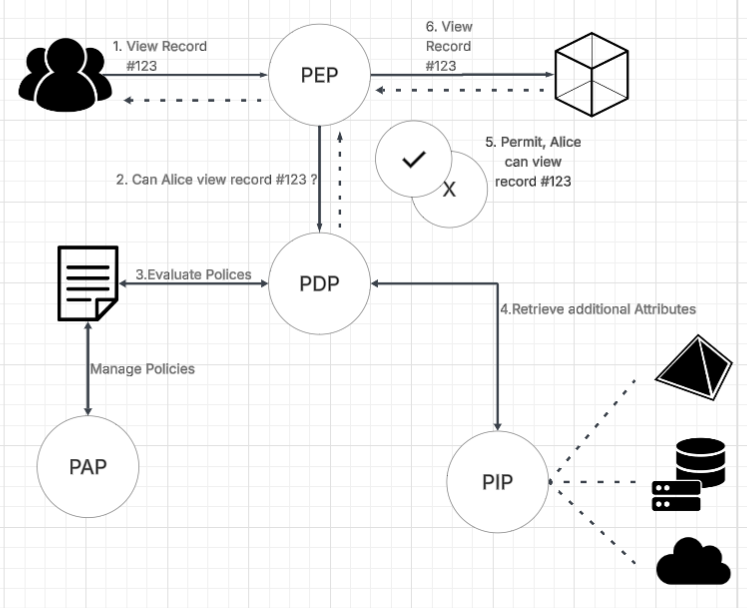
\includegraphics[width=0.75\linewidth]{images/abac.png}
    \caption{The standard architecture for ABAC}
    \label{fig:abac}
\end{figure}
However, ABAC also introduces operational challenges that become visible as policies and systems scale. First, ABAC is only as reliable as its attributes. If attributes such as shift status, ward assignment, care-team relationship, or record sensitivity are missing or outdated, decisions can be wrong even if the policy logic is correct. Second, ABAC tends to grow complex because policies often include many attribute predicates and combinations. \cite{Zheng2019ABAC} points out that ABAC policies become huge and complex in practice, making management difficult and conflicts frequent; they also emphasize that many real security failures come from policy misconfiguration rather than from cryptographic failures \cite{Zheng2019ABAC}. \cite{NIST800162Cost} similarly notes that ABAC is more complicated and therefore more costly to implement and maintain than simpler access control systems \cite{NIST800162Cost}.
\vspace{0.5cm}


One concrete problem that appears in large ABAC deployments is \textbf{policy conflict}. In simple terms, two or more rules may apply to the same request conditions but produce different decisions, which makes the overall behavior hard to predict and difficult to audit. \cite{Shu2009Conflicts} describe this clearly: conflicting rules make different assertions for the same set of user requests, and if conflicts are not detected and resolved, access control can become either too open or too restrictive \cite{Shu2009Conflicts}. Although some policy languages can use rule-combining strategies (e.g., deny-overrides), \cite{Shu2009Conflicts} warn that the result can be unpredictable when the rule set becomes too large to be comprehensible for administrators \cite{Shu2009Conflicts}. Because of this, conflict analysis is often treated as a \emph{pre-deployment} activity: detect conflicts early, fix them before policies are deployed into PDPs.


\subsubsection*{Policy conflict detection}
At a practical level, conflict detection methods aim to do three things:
\begin{enumerate}
    \item \textbf{Identify overlap:} find rules whose conditions can be satisfied by the same request (i.e., they overlap in the attribute space).
    \item \textbf{Check decision disagreement:} among overlapping rules, detect cases where the decision differs (permit vs deny).
    \item \textbf{Output actionable results:} return the pairs (or sets) of conflicting rules, often with supporting information such as which attribute predicates cause the overlap, so that a policy author can fix the policy.
\end{enumerate}

Because ABAC policies can contain many rules and many predicates, the key challenge is efficiency: a naive approach would compare every rule with every other rule and quickly becomes expensive.

\subsubsection*{Method A: Rule reduction + binary search (efficient pre-deployment detection)}
\textbf{Step 1 — Rule reduction (remove redundancy and normalize predicates):}  
The method starts from the observation that large policy sets contain redundancy: multiple rules may share attribute identifiers and overlapping ranges. Rule reduction transforms the original rules into a set of reduced rules whose attribute predicates do not intersect, while keeping the reduced policy \emph{semantically equivalent} to the original one \cite{Shu2009Conflicts}. The benefit is that conflict checking becomes more structured: the reduced rules are compact, and the method avoids repeatedly examining the same predicate patterns across many rules \cite{Shu2009Conflicts}.
\vspace{0.5cm}


\textbf{Step 2 — Binary search (find intersecting predicates efficiently)}  
After reduction, attribute predicates can be sorted, and binary search can be used to quickly identify which predicates intersect with a target predicate. The \cite{Shu2009Conflicts} paper explains that binary search becomes possible because non-intersection is guaranteed by the reduction step, allowing the search space to be halved repeatedly \cite{Shu2009Conflicts}. In implementation, the method also uses bitmap-based set operations for fast intersection/union of candidate rule sets \cite{Shu2009Conflicts}. 
\vspace{0.5cm}


The output is a list of statically-conflicting rules (conflicts detectable without executing real user requests), which can then be reviewed and corrected before deployment \cite{Shu2009Conflicts}. In other words, it supports administrators by turning a large, hard-to-read policy set into a smaller set of clear “conflict candidates”.

\subsubsection*{Method B: Binary sequence encoding + bitwise operations (fast overlap checking)}
This method encodes each ABAC rule into a set of binary sequences and then detects conflicts using bitwise AND operations \cite{Zheng2019ABAC}. The motivation is to improve efficiency when policies are large and complex. The paper explicitly states that the rule is transformed into binary sequences and conflicts are detected via AND operations, which improves detection efficiency \cite{Zheng2019ABAC}.  
\vspace{0.5cm}


Similar to Method A, the practical output is a set of detected conflicts among rules. The key advantage is speed: encoding and bitwise operations provide a computationally efficient way to test overlaps in the attribute space, which becomes useful when the rule set is large \cite{Zheng2019ABAC}.
\vspace{0.5cm}


ABAC provides a strong answer to dynamic hospital constraints because policies can directly reference context and relationships using attributes. At the same time, ABAC introduces new operational risks: attribute governance, policy complexity, and conflicts caused by overlapping rules. Conflict detection methods such as rule reduction + binary search, or binary sequence encoding + bitwise operations, are therefore useful as supporting tools to keep ABAC policies maintainable and safer before deployment \cite{ Zheng2019ABAC}.
\vspace{0.5cm}


These trade-offs lead naturally to hybrid RBAC/ABAC approaches. RBAC offers stability and organizational alignment, while ABAC offers context-sensitive precision. A hybrid model keeps the role structure as the baseline and uses ABAC constraints where hospital workflows require dynamic conditions.


\subsection{Hybrid RBAC/ABAC}
\label{sec:hybrid-rbac-abac}

RBAC and ABAC are often presented as two ends of the same spectrum. RBAC is strong when an organization already has a clear job structure, because administrators can reason in terms of job functions and stable responsibilities. ABAC is strong when access decisions must depend on the current situation, because policies can use subject, object, and environment attributes to express fine-grained rules. In real systems, especially in healthcare, the access control problem usually needs both: a stable role structure \emph{and} frequent context checks. This is the main motivation behind hybrid RBAC/ABAC models: they try to combine the administrative simplicity of RBAC with the expressive power of ABAC, without fully inheriting the weaknesses of either one \cite{KuhnCoyneWeil2010,Penelova2021HRABAC}.
\vspace{0.5cm}


Conceptually, a hybrid RBAC/ABAC decision can be viewed as a conjunction of two checks:

\[
\textit{Permit} \;\Leftrightarrow\; \underbrace{\textit{RBAC}(u,r,p)}_{\text{baseline eligibility}}
\;\wedge\;
\underbrace{\textit{ABAC}(s,o,a,e)}_{\text{contextual constraint}}
\]

where RBAC determines whether the user (or session) has an eligible role and permission, and ABAC evaluates attribute- and context-based conditions (e.g., IP, location, time, sensi tivity) before the permission is actually exercised. Depending on how roles and attributes are combined, the literature commonly distinguishes the following hybrid variants.
\vspace{0.5cm}


A hybrid model is not a single fixed architecture. It is a family of designs that connect roles and attributes in different ways. A useful way to think about hybridization is to ask: \emph{Where do roles end and where do attributes begin in the decision?} Some systems use attributes mainly to \emph{choose} roles, while others keep roles as the main structure and use attributes mainly to \emph{constrain} permissions. \cite{KuhnCoyneWeil2010} describes common RBAC-with-attributes directions (often called RBAC-A) and show that hybridization can reduce policy complexity compared to encoding everything as roles or everything as attribute rules \cite{KuhnCoyneWeil2010}. In other words, hybrid models are mostly about \emph{splitting the decision problem} so that each part is handled by the mechanism that fits it best. Across existing work, three practical hybrid patterns appear frequently.
\vspace{0.5cm}


First, \textbf{attribute-driven role activation (dynamic roles)} uses attributes to decide which roles are active for a user in a given session. The system keeps a role structure, but the role activation becomes context-dependent. This can reduce manual role switching and can be suitable when a small number of context variables controls access (e.g., on-site vs off-site). However, if the environment is rich in attributes, dynamic-role designs can quickly become hard to manage because many role activation combinations need to be considered \cite{KuhnCoyneWeil2010}.
\vspace{0.5cm}

\begin{figure} [H] 
    \centering
    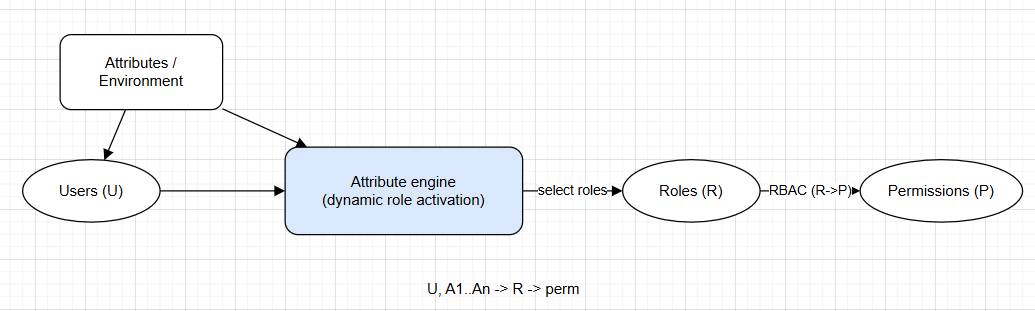
\includegraphics[width=0.75\linewidth]{images/dynamics-role.png}
    \caption{Attribute-driven role activation (dynamic roles) \cite{KuhnCoyneWeil2010}}
    \label{fig:dynamics-role}
\end{figure}

Second, \textbf{role-as-an-attribute (attribute-centric hybrids)} treats the role itself as one attribute among others. The access decision is computed by an ABAC-style policy engine, but one of the key attributes is the user’s job function or organizational position. This approach is conceptually simple because there is one evaluation mechanism (ABAC). The trade-off is that the policy layer can grow large, and the system may lose some of the practical benefits of RBAC administration (such as role hierarchy reasoning and simple permission reviews) unless the policy tooling is strong \cite{KuhnCoyneWeil2010}.
\begin{figure}[H]
    \centering
    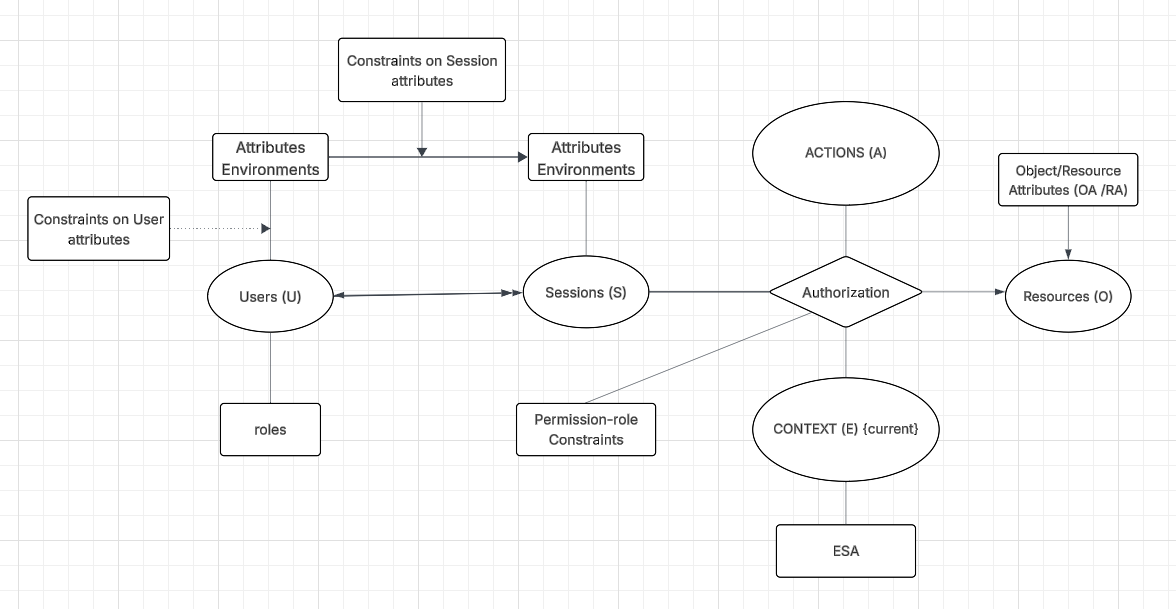
\includegraphics[width=0.75\linewidth]{images/attribute-centric.png}
    \caption{Attribute-centric (ABAC-first) hybrid model \cite{KuhnCoyneWeil2010}}
    \label{fig:placeholder}
\end{figure}


Third, \textbf{role-first with attribute constraints (role-centric hybrids)} starts from RBAC permissions but refines the decision using attributes. In this pattern, roles define the baseline permission set, and attributes act as constraints (for example, patient relationship, shift, location, data sensitivity, or emergency state). The key benefit is that organizations keep the familiar role hierarchy as the “main map” of responsibilities, while still enforcing fine-grained rules where needed \cite{KuhnCoyneWeil2010}. Many practical “RBAC + extra checks” implementations fall into this category; for example, Penelova proposes HRABAC as an extension of RBAC that adds attribute-based policy functions to protect data even when a role-level action is granted \cite{Penelova2021HRABAC}.
\begin{figure}[H]
    \centering
    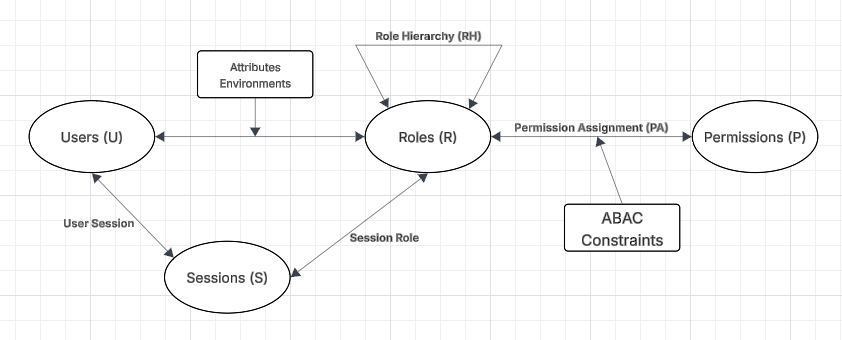
\includegraphics[width=0.75\linewidth]{images/role-centric.png}
    \caption{Role-centric (RBAC-first) hybrid model \cite{Houhou2024HyARBAC}}
    \label{fig:placeholder}
\end{figure}
Beyond RBAC-A, there are also \textbf{composite or layered designs} that explicitly combine multiple engines. One common form is a two-step decision: an RBAC step checks whether the action is allowed in principle for the user’s role, and an ABAC step then checks additional constraints. A cloud-oriented example is HyARBAC, which combines RBAC and ABAC so that access is not granted purely by role membership but also depends on attribute checks, aiming to improve flexibility while keeping RBAC’s administrative structure \cite{Houhou2024HyARBAC}. Layered hybrids are appealing in distributed systems because they naturally support separation of concerns: role administration can remain stable, while attribute policies evolve as business and compliance requirements change.
\vspace{0.5cm}


Hybridization does not automatically remove RBAC and ABAC problems; instead, it allows the system to apply \emph{targeted} solutions from each side.
\vspace{0.5cm}


From the RBAC side, role engineering (defining roles, hierarchies, and constraints) remains important because roles are still the main organizational structure in most hybrids. Role hierarchies and separation-of-duty constraints keep the baseline permissions consistent and reviewable. In a hybrid design, this baseline acts as the first control layer: it limits the maximum set of actions a user can attempt, which reduces the number of attribute rules that need to be evaluated for every request \cite{KuhnCoyneWeil2010}.
\vspace{0.5cm}


From the ABAC side, governance of attributes (where attributes come from, how they are validated, and how policies are maintained) becomes the main quality factor. Importantly, the policy-conflict detection techniques discussed in Section~2.2.2 become directly useful in hybrids as well. Even if RBAC defines the baseline permissions, the ABAC constraints still need to be correct and consistent. In practice, conflict detection in a hybrid model should do two things: (1) detect conflicts inside the attribute policy set itself (e.g., contradictory rules for the same request context), and (2) detect mismatches between role permissions and attribute constraints (e.g., a role grants an action broadly, but attribute rules deny it in almost all contexts, which may indicate a design error or a missing role refinement). Because the ABAC part is usually the more complex and more frequently updated part, applying conflict detection and policy validation there helps keep the entire hybrid model stable over time \cite{Houhou2024HyARBAC}.
\vspace{0.5cm}


This thesis targets an HMS deployed as a microservices-based application, where authorization must be both strict and operationally practical. In a hospital, job functions and reporting structure are stable and well understood (e.g., doctor, nurse, lab technician, pharmacist, receptionist). At the same time, real access needs are highly context-dependent: ward assignment, care-team relationship, shift schedule, emergency state, and data sensitivity can change frequently. For this reason, a hybrid model is a natural fit: it allows the system to keep a clear role baseline while enforcing the dynamic checks that appear in everyday clinical workflows.
\vspace{0.5cm}


Based on the hybrid patterns above, the implementation in this thesis will adopt a \emph{role-first hybrid approach} for the HMS, but only as the final design choice after reviewing the broader hybrid space. Concretely, roles will define the baseline permissions and the organizational hierarchy, while ABAC constraints will refine access for sensitive operations and patient-specific data access. This direction matches the hospital’s natural structure and supports clear auditing: administrators can still explain \emph{who is allowed to do what} at the role level, while the attribute layer explains \emph{under which conditions} the action is allowed. This choice also aligns with practical hybrid designs that extend RBAC with additional attribute-based checks to protect sensitive records \cite{KuhnCoyneWeil2010,Penelova2021HRABAC}.




\section{Microservices}
\label{sec:microservices}

\subsection{Definition of Microservices}
\label{sec:microservices-definition}
Microservices are commonly understood as an architectural style where an application is built as a set of small services that run independently and cooperate through lightweight communication. Each service is designed around a clear business capability, so teams can develop, test, and deploy services without having to ship the whole system at the same time. This is one of the main reasons microservices are often chosen for large domains like hospital management systems, where the system naturally splits into areas such as patient records, appointments, laboratory workflows, billing, and reporting.
\vspace{0.5cm}

In practice, microservices are less about “splitting code into many repositories” and more about setting boundaries that reduce tight coupling. A useful rule is that a service should hide its internal implementation details and expose only what other services need through an interface. This supports independent evolution: when one service changes internally, other services do not need to change as long as the interface remains compatible. Microservices are also typically associated with automation and fast release cycles, because small services are easier to build and deploy repeatedly than a large monolith \cite{BaresiGarriga2020,AbdelfattahCerny2022}.

\subsection{Design Principles of Microservices Architecture}
\label{sec:microservices-principles}
When building an application using microservices, the first practical step is choosing service boundaries. A common approach is to align services with business capabilities and keep each service scope “bounded”, meaning it owns a coherent part of the domain. This reduces cross-service dependencies and makes it realistic for teams to work in parallel. Once boundaries are defined, the architecture should aim for “share as little as possible” between services. Shared databases or shared internal libraries may look convenient at first, but they often recreate the same tight coupling that microservices are meant to avoid \cite{BaresiGarriga2020}.
\vspace{0.5cm}

The second step is defining how services communicate. In most microservice systems, service-to-service calls are implemented using lightweight mechanisms (for example REST APIs or messaging), with clear contracts. This contract-first mindset matters because it forces the system to be explicit about what data is exchanged and why. It also makes it easier to introduce versioning and gradual rollout strategies when interfaces evolve. In other words, microservices work well when services can tolerate change around them without breaking \cite{BaresiGarriga2020}.
\vspace{0.5cm}

The third step is enabling independent deployment through automation. Microservices are expected to be independently deployable, so the engineering workflow usually includes CI/CD pipelines, container-based packaging, and operational monitoring. The point is not the specific tool, but the capability: each service should be buildable, testable, and deployable on its own. This also implies that failures must be handled as normal conditions in distributed systems. Typical practices include health checks, timeouts, and resilience patterns to avoid one failing service causing a full-system outage \cite{AbdelfattahCerny2022,Yarygina2018}.
\vspace{0.5cm}

Finally, microservices require operational visibility. Because requests often pass through multiple services, teams need logging and monitoring that can follow a request across service boundaries. Without this, troubleshooting becomes difficult and security incidents become harder to investigate. As a result, observability is not an optional “nice-to-have” in microservices; it is part of what makes the architecture manageable \cite{AbdelfattahCerny2022}.

\subsection{Direct Connection to Hybrid Access Control}
\label{sec:microservices-hybrid-connection}
Microservices change the access control problem in a very direct way: instead of one application making one decision, there are many services making decisions across a request chain. If each microservice implements authorization rules in its own way, the system can quickly accumulate duplication and inconsistency. Prior work highlights a recognized need to apply security control policies consistently across microservices in the same system \cite{AbdelfattahCerny2022}.
\vspace{0.5cm}


A common architectural response is to use an API gateway as a controlled entry point. The gateway can act as a proxy and policy enforcement point that separates external clients from internal services, and it often takes responsibility for request routing and authentication at the edge \cite{AbdelfattahCerny2022}. However, edge checks alone are not sufficient for healthcare scenarios, because fine-grained authorization frequently depends on internal context (e.g., care-team relationship, ward assignment, emergency status). Therefore, authorization must remain enforceable at the service level as well.
\vspace{0.5cm}


This is where the connection to Hybrid RBAC/ABAC becomes natural. RBAC provides a stable baseline that matches hospital structure (roles such as doctor, nurse, lab technician), while ABAC provides the dynamic conditions that appear in real workflows (shift, location, patient consent, emergency override). In microservices, those decisions must also be consistent along the full request path. Research emphasizes that distributed components require propagating the user’s authentication and authorization identity throughout the full communication cycle, commonly using token-based mechanisms such as JWT \cite{AbdelfattahCerny2022,Yarygina2018}. This aligns well with a hybrid design where role information can be carried as a base claim, while required attributes can be fetched or evaluated when a service makes a decision.
\vspace{0.5cm}


In this thesis, these microservice properties motivate implementing authorization as a reusable capability rather than scattered logic: an authorization decision function (PDP-like) can be shared as a service, while each microservice acts as a local enforcement point (PEP-like) at the time it performs a sensitive operation. This structure supports consistent decisions, reduces duplicated rules, and keeps the access model aligned with the hospital’s role hierarchy while still handling dynamic clinical context \cite{AbdelfattahCerny2022}.



